            %\documentclass[a4,semhelv,landscape]{seminar}
\documentclass[landscape]{slides}
%\documentclass[pdf, default, slideBW, nocolorBG]{prosper}
\usepackage[left=1.0cm,top=0.2cm,right=1.0cm,nohead,nofoot]{geometry}
%\def\everyslide{\sffamily}
%\usepackage{fullpage}
\usepackage{graphicx}
\usepackage{setspace}
\usepackage{xcolor}
\usepackage{color}
\usepackage{fancyvrb}
\usepackage{verbatim}
\usepackage{nopageno}
%\usepackage{times}
% define some nice colors
\definecolor{myred}{rgb}{0.6,0,0}
\definecolor{myblue}{rgb}{0,0.2,0.4}
\def\imagetop#1{\vtop{\null\hbox{#1}}}
%\color{myblue}

%\DefineVerbatimEnvironment{sreoutput}{Verbatim}{fontsize=\scriptsize,xleftmargin=10.0\parindent}%
\DefineVerbatimEnvironment{sreoutput}{Verbatim}{fontsize=\small,xleftmargin=10.0\parindent}%
\DefineVerbatimEnvironment{sreoutput2}{Verbatim}{fontsize=\tiny,xleftmargin=10.0\parindent}%
%\input{macros}

\begin{document}
%%%%%%%%%%%%%%%%%%%%%%%%%%%%%%%%%%%%%%%%%%%%%%%%%%%%%%%%%%%%%%%%%%%%%%%%%%
\begin{slide}

\center{\large{\textbf{Searching for novel group I introns}}}
\normalsize

02.03.15

\medskip

%\includegraphics[width=3in]{figs/ssualign-logo}

\small

%\begin{tabular}{c}
%Janelia Farm Research Campus \\
%Howard Hughes Medical Institute \\ 
%\\
%Deparment of Genetics \\
%Washington University in St. Louis \\
%\\
%%& & Washington University in St. Louis \\
%\end{tabular}%
%
%\includegraphics[width=2.25in]{figs/janelia}
%\hspace{2in}
%\includegraphics[width=1.75in]{figs/washu}

%\end{center}
\end{slide}
%%%%%%%%%%%%%%%%%%%%%%%%%%%%%%%%%%%%%%%%%%%%%%%%%%%%%%%%%%%%%%%%%%%%%%%%%%
\begin{slide}
\center{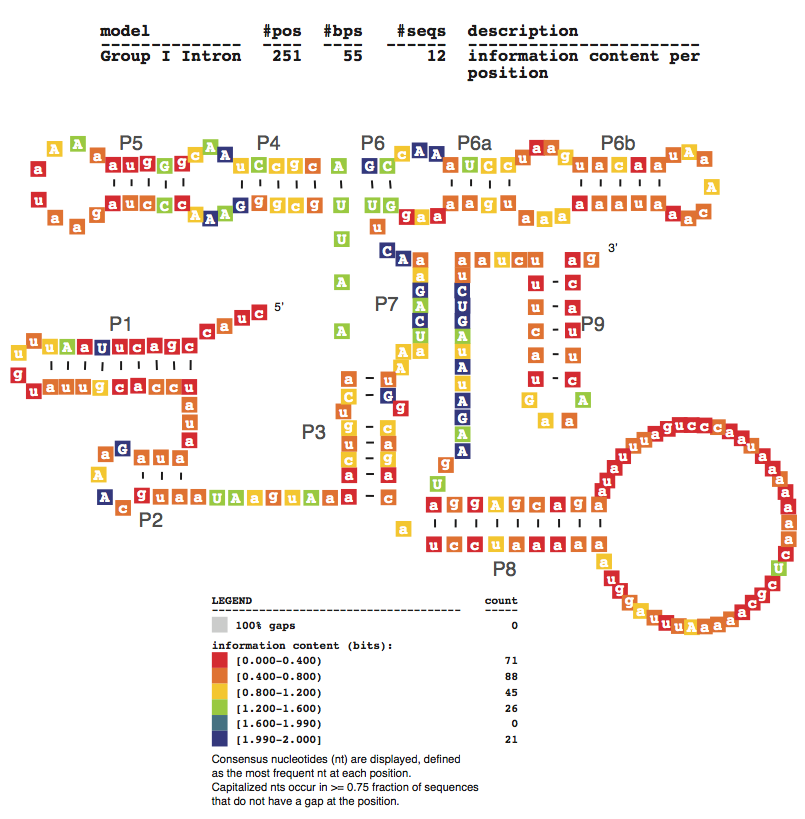
\includegraphics[height=8in]{figs/RF00028-ss-info-ss-1}}
\vfill
\end{slide}
%%%%%%%%%%%%%%%%%%%%%%%%%%%%%%%%%%%%%%%%%%%%%%%%%%%%%%%%%%%%%%%%%%%%%%%%%%
\begin{slide}
\center{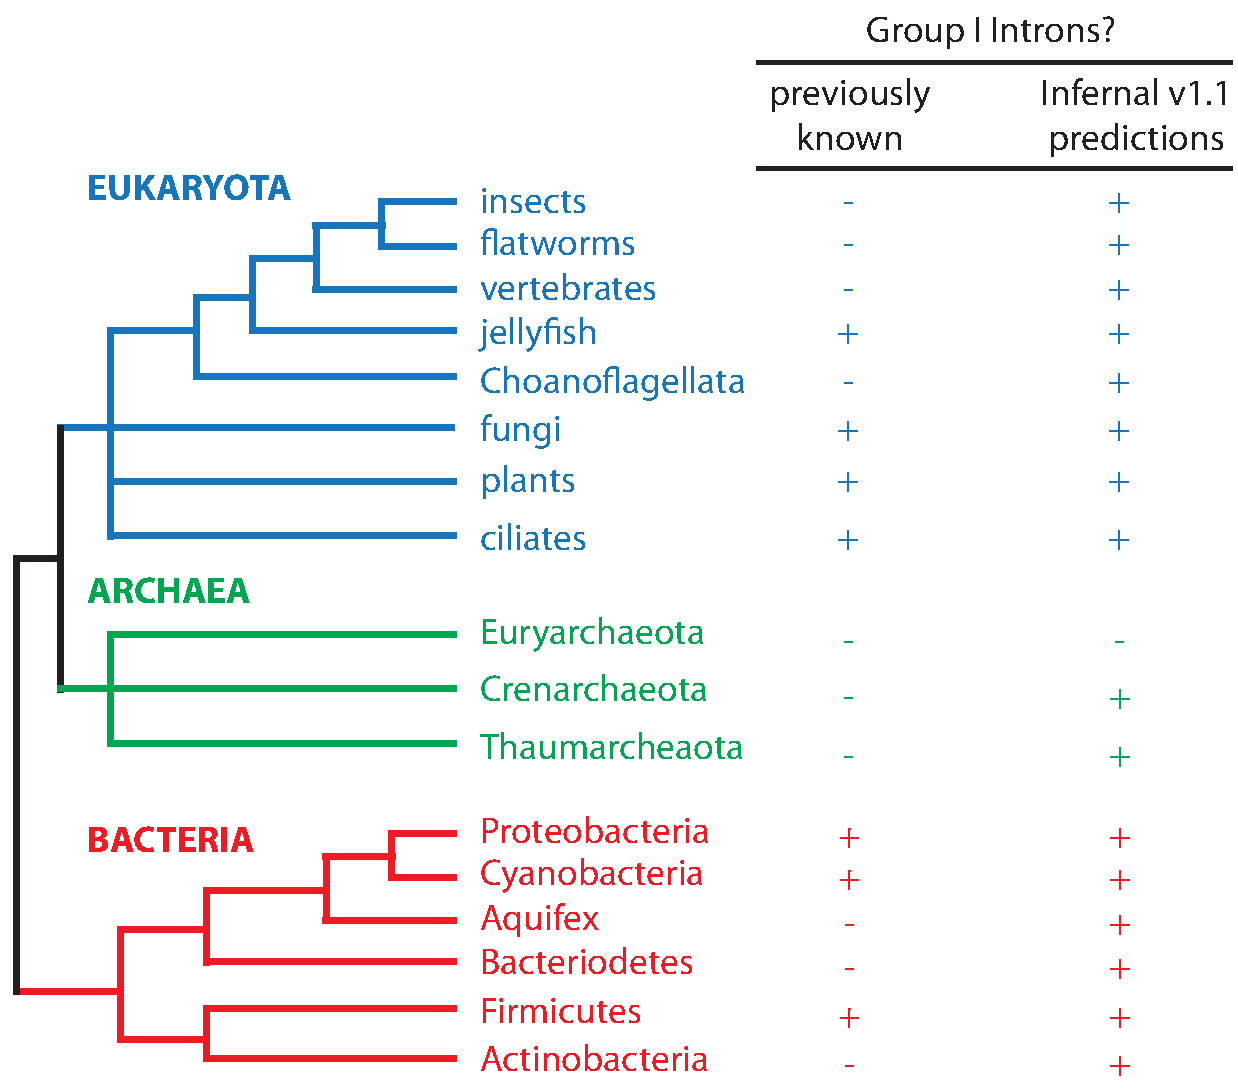
\includegraphics[height=8in]{figs/sean-slide-012215-gp1i-distro}}
\vfill
\end{slide}
%%%%%%%%%%%%%%%%%%%%%%%%%%%%%%%%%%%%%%%%%%%%%%%%%%%%%%%%%%%%%%%%%%%%%%%%%%
\begin{slide}
\begin{center}
\small
\textbf{GISSD: Group I Intron Sequence and Structure Database}
\end{center}

\center{
\includegraphics[width=10in]{figs/gissd-banner}}

\center{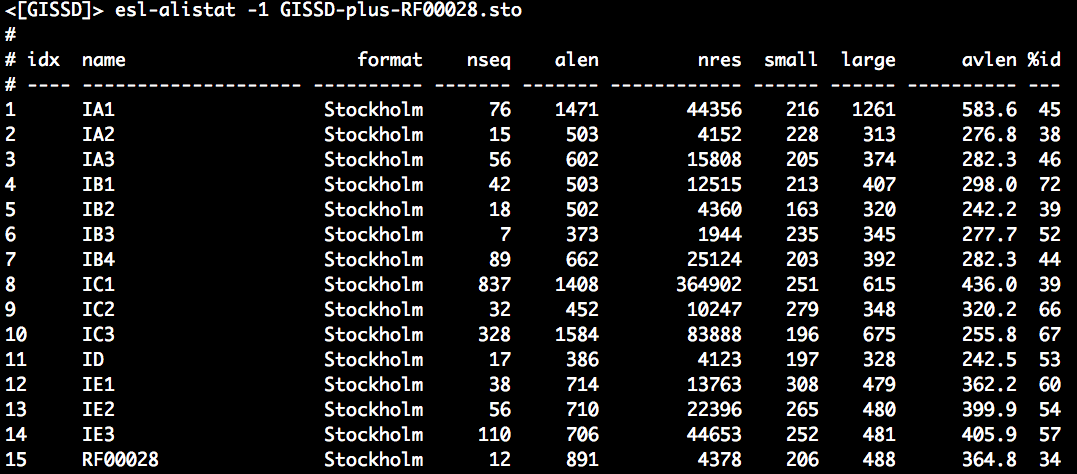
\includegraphics[width=10in]{figs/gissd-alistat-ss-1}}

\vfill
\end{slide}
%%%%%%%%%%%%%%%%%%%%%%%%%%%%%%%%%%%%%%%%%%%%%%%%%%%%%%%%%%%%%%%%%%%%%%%%%%
\begin{slide}
\begin{center}
\small
\textbf{Measuring specificity of GISSD models against training
  sequences using RNAVORE} 
\end{center}
%\center{\includegraphics[width=10in]{figs/gissd-specificity-ss-1-PRESENTED-INCORRECT}}
\center{\includegraphics[width=10in]{figs/gissd-specificity-ss-1}}
\vfill
\end{slide}
%%%%%%%%%%%%%%%%%%%%%%%%%%%%%%%%%%%%%%%%%%%%%%%%%%%%%%%%%%%%%%%%%%%%%%%%%%
\begin{slide}
\begin{center}
\small
\textbf{Searching Rfamseq with GISSD models}
\end{center}

\small
\begin{center}
\begin{tabular}{l|r|rrr|r}
\tt
        & \# RF00028 & \# hits   & \# hits& \# hits& total     \\
type    & seed seqs  & total     & common & unique & CPU hours \\ \hline
IA1     & 3          &  814      & 385    & 425    & 1076 \\
IA2     & 1          &  1722     & 823    & 899    & 50 \\
IA3     &            &   958     & 401    & 557    & 14 \\
IB1     &            &  3949     & 1033   & 2916   & 32 \\
IB2     &            & 1861     & 467    & 1394   & 31 \\
IB3     &            & 479     & 136    & 343    & 40 \\
IB4     &  1         & 5717     & 2400   & 3317   & 39 \\
IC1     &  3         & 8475     & 5385   & 3090   & 24 \\
IC2     &            & 4870     & 3858   & 1012   & 22 \\
IC3     & 4          & 72692     & 66033  & 6659   & 136 \\
ID      &            & 572     & 0      & 572    & 29 \\
IE1     &            & 1305     & 10     & 1295   & 12 \\
IE2     &            & 1377     & 8      & 1369   & 12 \\
IE3     &            & 1379     & 1      & 1378   & 13 \\
        &            &          &        &        &    \\
total   & 12         & 106170*   & 80940* & 25226  & 1530 \\
        &           &           &        &    \\
RF00028 & -         & 71421     & 71421  & -      & 125 \\
\end{tabular}

\begin{description}
\item[*] contains overlaps
\end{description}

\end{center}

\vfill
\end{slide}
%%%%%%%%%%%%%%%%%%%%%%%%%%%%%%%%%%%%%%%%%%%%%%%%%%%%%%%%%%%%%%%%%%%%%%%%%
\begin{slide}
\begin{center}
\small
\textbf{Phylogenetic distribution of GISSD hits - viruses, bacteria
  and archaea}
\end{center}

\center{\includegraphics[width=10in]{figs/1e-5-table-noneuks}}

\vfill
\end{slide}
%%%%%%%%%%%%%%%%%%%%%%%%%%%%%%%%%%%%%%%%%%%%%%%%%%%%%%%%%%%%%%%%%%%%%%%%%
\begin{slide}
\begin{center}
\small
\textbf{Phylogenetic distribution of GISSD hits - eukarya}
\end{center}

\center{\includegraphics[width=10in]{figs/1e-5-table-euks}}

\vfill
\end{slide}
%%%%%%%%%%%%%%%%%%%%%%%%%%%%%%%%%%%%%%%%%%%%%%%%%%%%%%%%%%%%%%%%%%%%%%%%%
\begin{slide}
\begin{center}
\textbf{Strategy for investigation of vertebrate hits}
\end{center}

\small
\begin{itemize}
\item Align each hit to its best matching GISSD model.
\item Use that single sequence alignment as a SEED for a search
  against Rfamseq.
\end{itemize}
\begin{itemize}
\item Possible outcomes:
\begin{itemize}
\item Novel hit, unlike all known group Is: most top hits are in
  related organisms
\item Contamination, misannotated: many nearly identical hits far away
  on tree
\end{itemize}
\end{itemize}

\vfill
\end{slide}
%%%%%%%%%%%%%%%%%%%%%%%%%%%%%%%%%%%%%%%%%%%%%%%%%%%%%%%%%%%%%%%%%%%%%%%%%
\begin{slide}
\begin{center}
\textbf{First group to investigate: vertebrates}
\end{center}

\center{An example hit in human}
\center{\includegraphics[width=10in]{figs/human-example-species}}

\vfill
\end{slide}
%%%%%%%%%%%%%%%%%%%%%%%%%%%%%%%%%%%%%%%%%%%%%%%%%%%%%%%%%%%%%%%%%%%%%%%%%
\begin{slide}
\begin{center}
\textbf{Summarizing vertebrate single sequence searches}
\end{center}

\center{\includegraphics[width=10in]{figs/vertebrate-table2}}

All but four IB4 candidates and one ID candidates are almost certainly
contamination.

\vfill
\end{slide}
%%%%%%%%%%%%%%%%%%%%%%%%%%%%%%%%%%%%%%%%%%%%%%%%%%%%%%%%%%%%%%%%%%%%%%%%%
\begin{slide}
\begin{center}
\textbf{Remaining 5 hits are in the cichlid Rhamphochromis esox}
\end{center}

\begin{itemize}
\item These are all probably contamination:
\begin{itemize}
\item one was 100\% identical to a plant sequence
\item two were clearly mitochondrial fungal sequence (protein
  homology)
\item two were judged probably fungal due to similarity to other
  fungal group Is.
\end{itemize}
\end{itemize}

\vfill
\end{slide}
%%%%%%%%%%%%%%%%%%%%%%%%%%%%%%%%%%%%%%%%%%%%%%%%%%%%%%%%%%%%%%%%%%%%%%%%%
\begin{slide}
\begin{center}
\textbf{2nd group to investigate: archaea}
\end{center}

\center{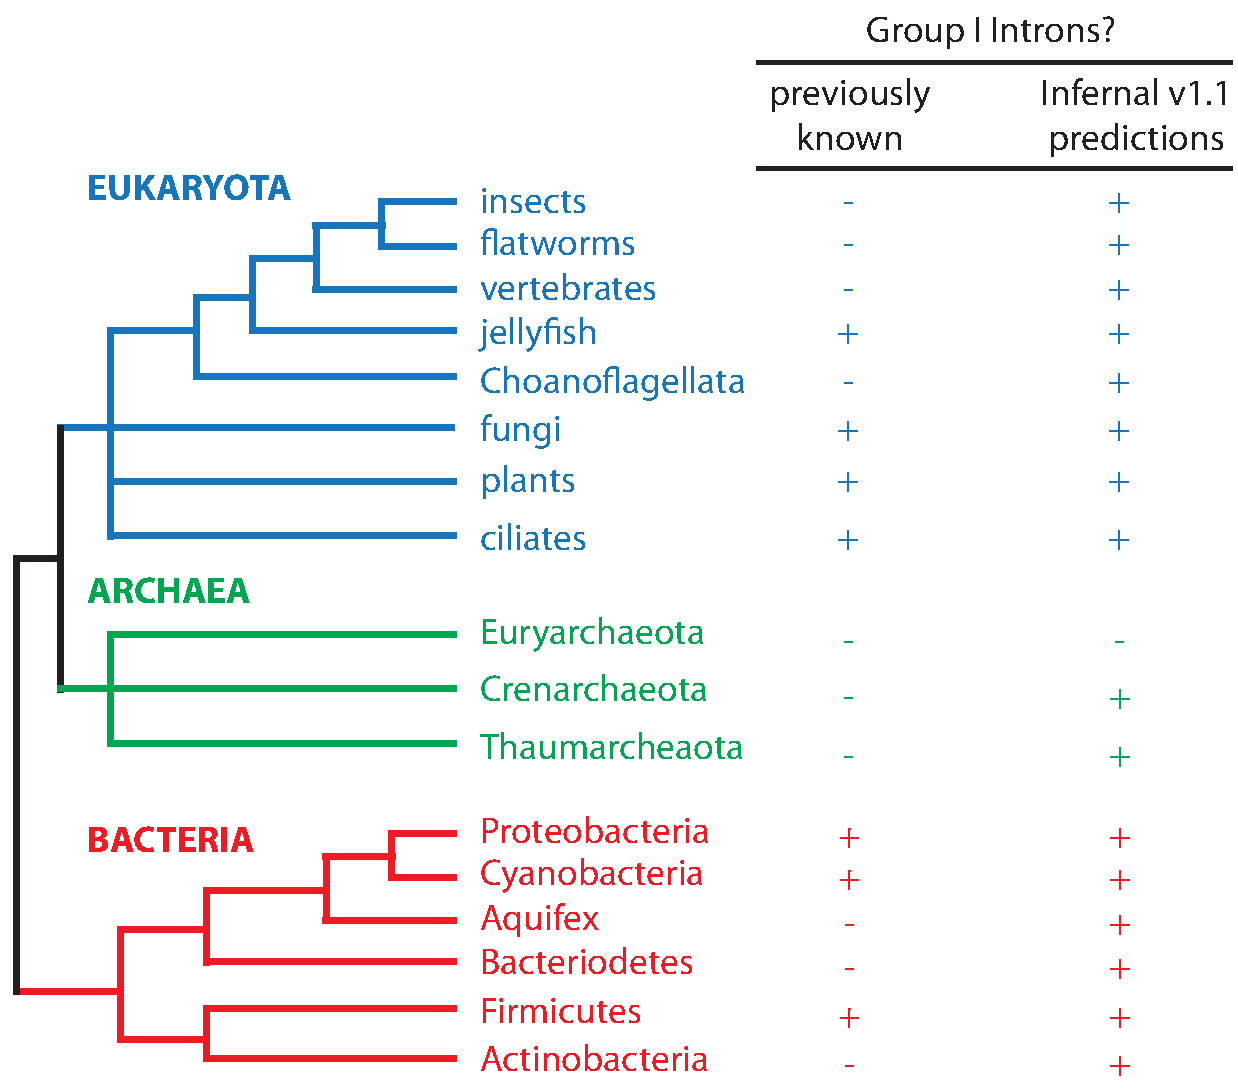
\includegraphics[height=8in]{figs/sean-slide-012215-gp1i-distro}}

\vfill
\end{slide}
%%%%%%%%%%%%%%%%%%%%%%%%%%%%%%%%%%%%%%%%%%%%%%%%%%%%%%%%%%%%%%%%%%%%%%%%%
\begin{slide}
\begin{center}
\textbf{Annotation of crenarchaeota candidate}
\end{center}

\center{\includegraphics[width=10in]{figs/arc-1-gene-diagram}}

\vfill
\end{slide}
%%%%%%%%%%%%%%%%%%%%%%%%%%%%%%%%%%%%%%%%%%%%%%%%%%%%%%%%%%%%%%%%%%%%%%%%%
\begin{slide}
\begin{center}
\textbf{Annotation of thaumarchaeota candidate}
\end{center}

\center{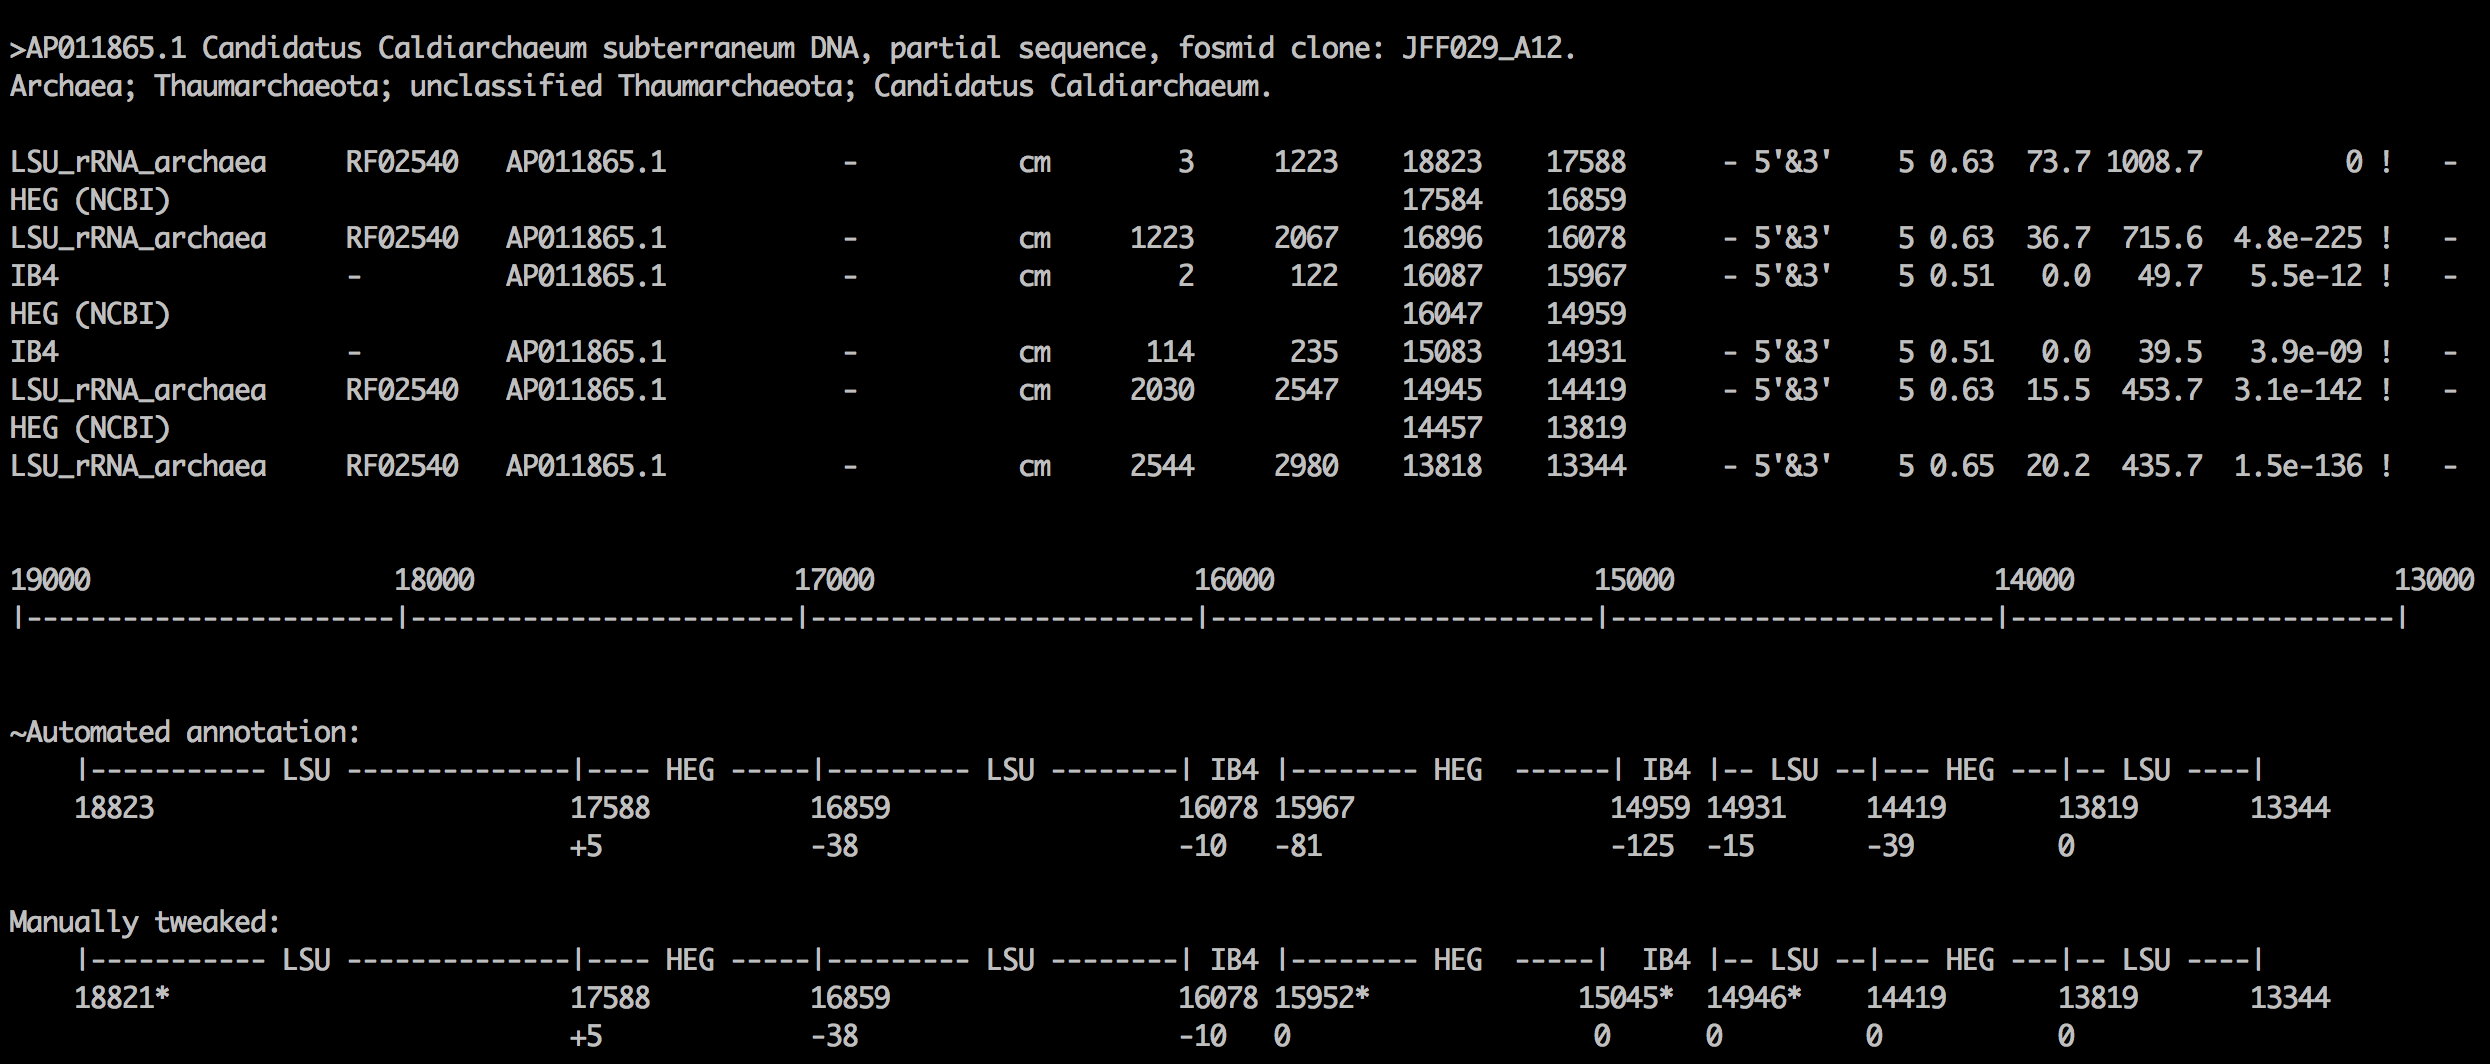
\includegraphics[width=10in]{figs/arc-2-gene-diagram}}

\vfill
\end{slide}
%%%%%%%%%%%%%%%%%%%%%%%%%%%%%%%%%%%%%%%%%%%%%%%%%%%%%%%%%%%%%%%%%%%%%%%%%
\begin{slide}
\begin{center}
\textbf{Thaumarchaeota group I structure}
\end{center}

\center{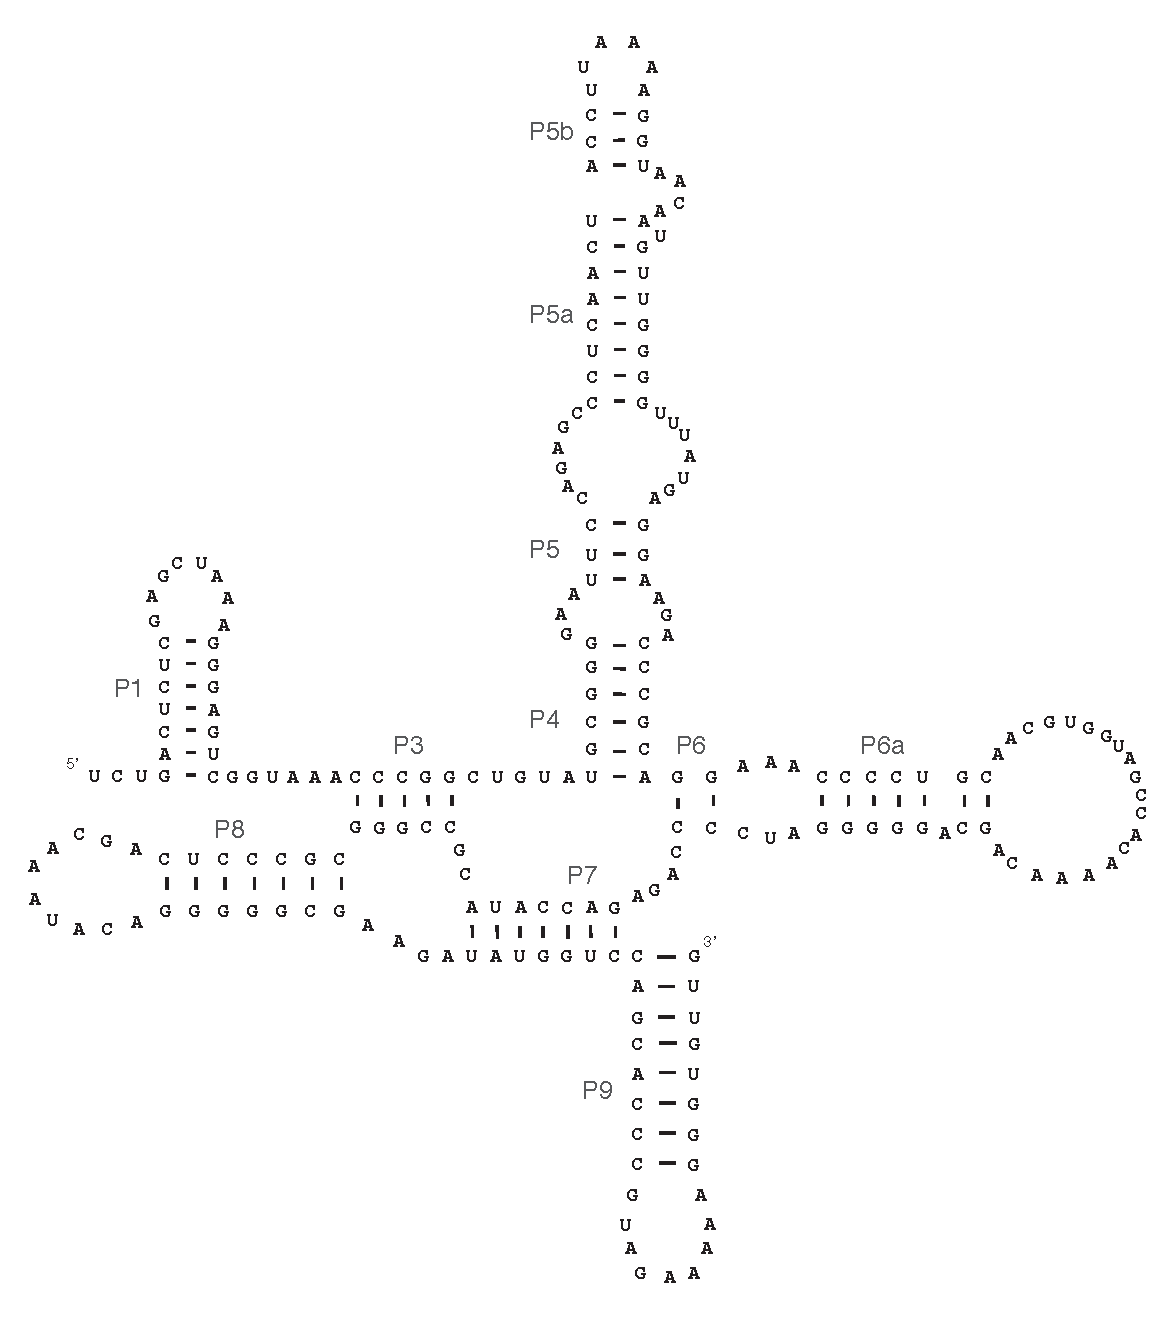
\includegraphics[height=6.5in]{figs/thaumarchaea-AP011865-1-classic-coke}}

\vfill
\end{slide}
%%%%%%%%%%%%%%%%%%%%%%%%%%%%%%%%%%%%%%%%%%%%%%%%%%%%%%%%%%%%%%%%%%%%%%%%%
\begin{slide}
\begin{center}
\small
\textbf{Phylogenetic distribution of GISSD hits - eukarya}
\end{center}

\center{\includegraphics[width=10in]{figs/1e-5-table-euks}}

\vfill
\end{slide}
%%%%%%%%%%%%%%%%%%%%%%%%%%%%%%%%%%%%%%%%%%%%%%%%%%%%%%%%%%%%%%%%%%%%%%%%%
\begin{slide}
\small
\center{\includegraphics[height=8.5in]{figs/euk-phylogeny-RF00028-counts-110314-1}}
\vfill
\end{slide}
%%%%%%%%%%%%%%%%%%%%%%%%%%%%%%%%%%%%%%%%%%%%%%%%%%%%%%%%%%%%%%%%%%%%%%%%%%
\begin{slide}
\begin{center}
\textbf{Platyhelminthes}
\end{center}

\center{\includegraphics[width=10in]{figs/platyhelminthes-fulltable}}

\vfill
\end{slide}
%%%%%%%%%%%%%%%%%%%%%%%%%%%%%%%%%%%%%%%%%%%%%%%%%%%%%%%%%%%%%%%%%%%%%%%%%
\begin{slide}
\begin{center}
\textbf{Arthropoda}
\end{center}

\center{\includegraphics[width=10in]{figs/arthropoda-fulltable}}

\vfill
\end{slide}
%%%%%%%%%%%%%%%%%%%%%%%%%%%%%%%%%%%%%%%%%%%%%%%%%%%%%%%%%%%%%%%%%%%%%%%%%
\begin{slide}
\begin{center}
\textbf{Cnidaria}
\end{center}

\center{\includegraphics[width=10in]{figs/cnidaria-fulltable}}

\vfill
\end{slide}
%%%%%%%%%%%%%%%%%%%%%%%%%%%%%%%%%%%%%%%%%%%%%%%%%%%%%%%%%%%%%%%%%%%%%%%%%
\begin{slide}
\begin{center}
\textbf{Placozoa}
\end{center}

\center{\includegraphics[width=10in]{figs/placozoa-fulltable}}

\vfill
\end{slide}
%%%%%%%%%%%%%%%%%%%%%%%%%%%%%%%%%%%%%%%%%%%%%%%%%%%%%%%%%%%%%%%%%%%%%%%%%
\begin{slide}
\begin{center}
\textbf{Ctenophora}
\end{center}

\center{\includegraphics[width=10in]{figs/ctenophora-fulltable}}

\vfill
\end{slide}
%%%%%%%%%%%%%%%%%%%%%%%%%%%%%%%%%%%%%%%%%%%%%%%%%%%%%%%%%%%%%%%%%%%%%%%%%
\begin{slide}
\begin{center}
\textbf{Demospongiae}
\end{center}

\center{\includegraphics[width=10in]{figs/demospongiae-fulltable}}

\vfill
\end{slide}
%%%%%%%%%%%%%%%%%%%%%%%%%%%%%%%%%%%%%%%%%%%%%%%%%%%%%%%%%%%%%%%%%%%%%%%%%
\begin{slide}
\begin{center}
\textbf{Choanoflagellata}
\end{center}

\center{\includegraphics[width=10in]{figs/choano-fulltable}}

\vfill
\end{slide}
%%%%%%%%%%%%%%%%%%%%%%%%%%%%%%%%%%%%%%%%%%%%%%%%%%%%%%%%%%%%%%%%%%%%%%%%%
\begin{slide}
\begin{center}
\textbf{Ichthyosporea}
\end{center}

\center{\includegraphics[width=10in]{figs/ichthy-fulltable}}

\vfill
\end{slide}
%%%%%%%%%%%%%%%%%%%%%%%%%%%%%%%%%%%%%%%%%%%%%%%%%%%%%%%%%%%%%%%%%%%%%%%%%
\begin{slide}
\begin{center}
\textbf{Apusozoa}
\end{center}

\center{\includegraphics[width=10in]{figs/apusozoa-fulltable}}

\vfill
\end{slide}
%%%%%%%%%%%%%%%%%%%%%%%%%%%%%%%%%%%%%%%%%%%%%%%%%%%%%%%%%%%%%%%%%%%%%%%%%
\begin{slide}
\begin{center}
\small
\textbf{Phylogenetic distribution of GISSD hits - viruses, bacteria
  and archaea}
\end{center}

\center{\includegraphics[width=10in]{figs/1e-5-table-noneuks}}

\vfill
\end{slide}
%%%%%%%%%%%%%%%%%%%%%%%%%%%%%%%%%%%%%%%%%%%%%%%%%%%%%%%%%%%%%%%%%%%%%%%%%
\begin{slide}
\begin{center}
\small
\textbf{Phylogenetic distribution of GISSD hits - eukarya}
\end{center}

\center{\includegraphics[width=10in]{figs/1e-5-table-euks}}

\vfill
\end{slide}
%%%%%%%%%%%%%%%%%%%%%%%%%%%%%%%%%%%%%%%%%%%%%%%%%%%%%%%%%%%%%%%%%%%%%%%%%


\end{document}

